\chapter{\uppercase{Modified Interior Penalty on Arbitrary Polygonal Cells}}
\label{mip_chapter}
\section{Introduction}
In Chapter \ref{anmg_chapter}, we saw that at the coarsest level of ANMG a Diffusion
Synthetic Acceleration needs to be solved. DSA is very often used to speed up the
calculation when the scattering is isotropic or weakly anisotropic. This is
because the transport sweep attenuates the quickly varying error modes whereas
the diffusion operator attenuates the slowly varying error modes.  Another
important property of the diffusion operator is that it is easily inverted. 
In this Chapter, we introduce the Modified Interior Penalty (MIP) DSA on arbitrary 
polygonal mesh. Several discretization methods haven been developed for 
arbitrary polygonal meshes \cite{pwld_3d,pwl_diffusion,palmer_fe,mimetic,
cell_centered_diff,palmer_proc,palmer_ane,pwld_2d,wachspress}. Using polygonal 
cells can be advantageous because the number of unknowns can be reduced while 
maintaining symmetry within the mesh. This potential reduction in the number of 
unknowns can be seen by comparing a hexagonal cell with a triangular 
discretization of the same area:
\begin{figure}[H]
\centering
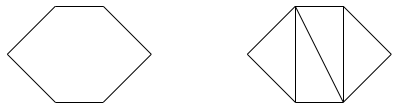
\includegraphics[width=0.5\textwidth]{./Dsa/hex_tri_cells}
\caption{Hexagonal cell versus triangle cells.}
\end{figure}
If there is one unknown per vertex, the hexagonal cell will have only six
unknowns compared to the twelve unknowns of the triangular discretization. Another 
advantage of polygonal cells is that they can be used for adaptive mesh 
refinement (AMR) \cite{amr_block,amr_rad,amr_unstruc} without having to
deal with hanging nodes \cite{locally_hanging_nodes,arbitrary_hanging_nodes,
dealII_hanging_nodes}. On the figure below, the left cell is a pentagon 
whereas the two cells on the right are quadrilaterals:
\begin{figure}[H]
\centering
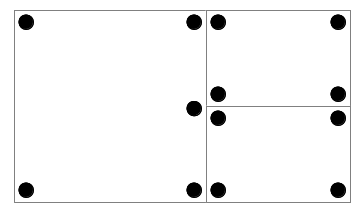
\includegraphics[width=0.3\textwidth]{./Dsa/amr}
\caption{AMR mesh.}
\end{figure}
Among the different discretization schemes for polygonal meshes, the PieceWise 
Linear Discontinuous (PWLD) finite elements \cite{pwld_3d,pwld_2d} 
have been successfully used to solve the transport equation on arbitrary
polygonal meshes. Another variant of the PieceWise Linear finite elements, the
PieceWise Linear Continuous finite elements were also developed and used 
to discretize the diffusion equation. They have shown to be a second order
accuracy method and to produce a symmetric and positive definite matrix 
\cite{pwl_diffusion} contrarily to others discretization for arbitrary
polygonal meshes \cite{pwl_diffusion}. However, no DSA 
\cite{dsa_ref,larsen_dsa,consistent_p1} was developed using PWLD finite
elements. In this work, we remedy this lack by adapting the Modified Interior 
Penalty (MIP) DSA developed in \cite{mip} for triangular cells. By using PWLD 
finite elements with MIP, MIP will be able to to be used on arbitrary polygonal 
cells. Since MIP produces SPD equations, it has usually been solved using conjugate 
gradient preconditioned by SSOR. In this work, the effectiveness of algebraic 
multigrid methods (AMG) to precondition the Krylov solver \cite{amg,amg_course} 
will be tested. Algebraic multigrid methods allow to use multigrid techniques 
when there is no grid or when the mesh is unstructured. Instead of using a 
succession of grids based on the geometry of the problems, the grids are based 
on properties of the matrix. Therefore, AMG can be used as black-box solver or 
preconditioner.
